\documentclass[xcolor=table]{beamer}
% generated by Madoko, version 1.1.3
%mdk-data-line={1}


\usepackage[heading-base={2},section-num={False},bib-label={hide},fontspec={True}]{madoko2}
%mdk-data-line={1;out\presentation.mdk:79}

    \ifbeamer\relax\else
      \providecommand{\usetheme}[2][]{}
      \providecommand{\usecolortheme}[2][]{}
      \providecommand{\usefonttheme}[2][]{}
      \providecommand{\pause}[1][]{}
      \providecommand{\AtBeginSection}[2][]{}
      \providecommand{\AtBeginSubsection}[2][]{}
      \providecommand{\AtBeginSubsubsection}[2][]{}
      \providecommand{\AtBeginPart}[2][]{}
      \providecommand{\AtBeginLecture}[2][]{}
      \providecommand{\theoremstyle}[2][]{}
      \makeatletter
      \def\newtheorem{\@ifstar\newtheoremx\newtheoremx}
      \makeatother
      \providecommand{\newtheoremx}[3][]{}{}
    \fi
%mdk-data-line={1;out\presentation.mdk:96}

    \ifbeamer\usetheme[]{singapore}\fi
\begin{document}



%mdk-data-line={8}
%mdk-data-line={8}
%mdk-data-line={9}
\mdxtitleblockstart{}
%mdk-data-line={9}
\mdxtitle{{\mdfontsize{3em}\mdline{9}Particiones balanceadas de conjuntos geometricos 3 coloreados en el plano}}%mdk
\mdxauthorstart{\Large{}
%mdk-data-line={14}
\mdxauthorname{{\mdfontsize{1.4em}\mdline{14}Bereg, Hurtado, Kano, Korman, Lara, Seara, et al.~(\mdcite{bereg201521}{2015})}}%mdk
}\mdxauthorend\mdtitleauthorrunning{}{}\mdxtitleblockend%mdk

%mdk-data-line={11}
\begin{mdframe}%mdk

\frametitle{Contenido}\label{heading-sec-contenido}%mdk%mdk
\mdline{12}
\begin{mdtoc}%mdk

\begin{mdtocblock}%mdk

\mdtocitemx{sec-contenido}{\mdref{sec-contenido}{1.\hspace*{0.5em}Contenido}}%mdk

\mdtocitemx{sec-definiciones}{\mdref{sec-definiciones}{2.\hspace*{0.5em}Definiciones}}%mdk

\mdtocitemx{sec-equiparticion}{\mdref{sec-equiparticion}{3.\hspace*{0.5em}Equiparticion}}%mdk

\mdtocitemx{sec-celdas-el-arreglos-coloreados}{\mdref{sec-celdas-el-arreglos-coloreados}{4.\hspace*{0.5em}Celdas el arreglos coloreados}}%mdk

\begin{mdtocblock}%mdk

\mdtocitemx{sec-en-el-plano}{\mdref{sec-en-el-plano}{4.1.\hspace*{0.5em}En el plano}}%mdk

\mdtocitemx{sec-en-dimensiones-ms-grandes}{\mdref{sec-en-dimensiones-ms-grandes}{4.2.\hspace*{0.5em}En dimensiones más grandes}}%mdk
%mdk
\end{mdtocblock}%mdk

\mdtocitemx{sec-conjunto-de-puntos-3-coloreados-y-cuas-balanceadas}{\mdref{sec-conjunto-de-puntos-3-coloreados-y-cuas-balanceadas}{5.\hspace*{0.5em}Conjunto de puntos 3 coloreados y cuñas balanceadas}}%mdk

\mdtocitemx{sec-particiones-balanceadas-en-curvas-cerradas-de-jordan}{\mdref{sec-particiones-balanceadas-en-curvas-cerradas-de-jordan}{6.\hspace*{0.5em}Particiones balanceadas en curvas cerradas de Jordan}}%mdk

\mdtocitemx{sec-l-lineas-en-el--lattice-}{\mdref{sec-l-lineas-en-el--lattice-}{7.\hspace*{0.5em}$L$-lineas en el \emph{lattice}}}%mdk

\mdtocitemx{sec-bibliografia}{\mdref{sec-bibliografia}{8.\hspace*{0.5em}Bibliografia}}%mdk

\mdtocitemx{sec-bibliography}{\mdref{sec-bibliography}{References}}%mdk
%mdk
\end{mdtocblock}%mdk
%mdk
\end{mdtoc}%mdk
%mdk
\end{mdframe}\label{sec-contenido}%mdk%mdk

%mdk-data-line={14}
\begin{mdframe}%mdk

\frametitle{Definiciones}\label{heading-sec-definiciones}%mdk%mdk

%mdk-data-line={15}
\begin{mdbmarginx}{1ex}{0pt}{1ex}{0pt}%mdk
%mdk-data-line={16}
\begin{onlyenv}<+->%mdk
\noindent\mdline{16}\textbf{Definition~1.} \mdbr
\mdline{16}  Sea \mdline{16}$S$\mdline{16} un conjunto finitos de objetos geometricos particionados en clases o \mdline{16}\emph{colores}\mdline{16}.
  Sea \mdline{17}$S'\subseteq S$\mdline{17} decimos que esta \mdline{17}\textbf{balanceado}\mdline{17} si contiene la misma cantidad de elementos
  de \mdline{18}$S$\mdline{18} de cada uno de los colores.%mdk
\end{onlyenv}%mdk%mdk
\end{mdbmarginx}%mdk

%mdk-data-line={21}
\begin{mdbmarginx}{1ex}{0pt}{1ex}{0pt}%mdk
%mdk-data-line={22}
\begin{onlyenv}<+->%mdk
\noindent\mdline{22}\textbf{Definition~2.} ({\itshape Arreglo Simple})\mdbr
\mdline{22}  Dado el arreglo, este no contiene lineas paralelas y no mas de dos lineas intersectan
  en un punto%mdk
\end{onlyenv}%mdk%mdk
\end{mdbmarginx}%mdk
%mdk
\end{mdframe}\label{sec-definiciones}%mdk%mdk

%mdk-data-line={27}
\begin{mdframe}%mdk

\frametitle{Equiparticion}\label{heading-sec-equiparticion}%mdk%mdk
%mdk
\end{mdframe}\label{sec-equiparticion}%mdk%mdk

%mdk-data-line={31}
\begin{mdframe}%mdk

%mdk-data-line={32}
\noindent\mdline{32}  Es posible que dado un conjunto tricolor de puntos en plano no se pueda encontrar
  ninguna linea \mdline{33}\emph{no trivial}\mdline{33} que divida al plano%mdk
%mdk
\end{mdframe}%mdk

%mdk-data-line={35}
\begin{mdframe}%mdk

%mdk-data-line={36}
\noindent\mdline{36}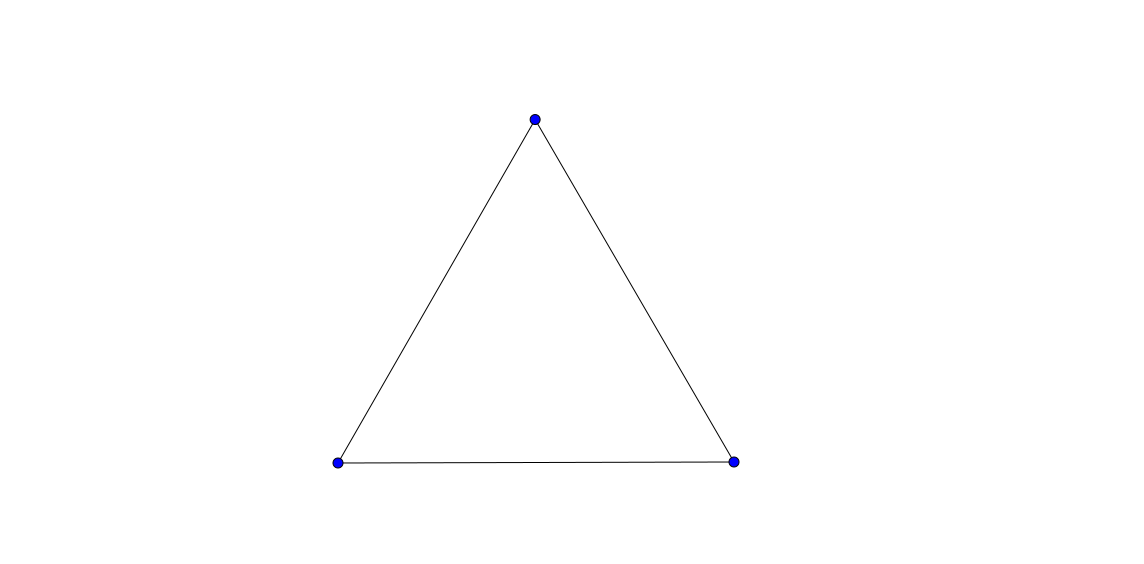
\includegraphics[keepaspectratio=true,width=\dimwidth{1.00},height=\dimheight{1.00}]{images/non_trivial_cut00}{}%mdk
%mdk
\end{mdframe}%mdk

%mdk-data-line={38}
\begin{mdframe}%mdk

%mdk-data-line={39}
\noindent\mdline{39}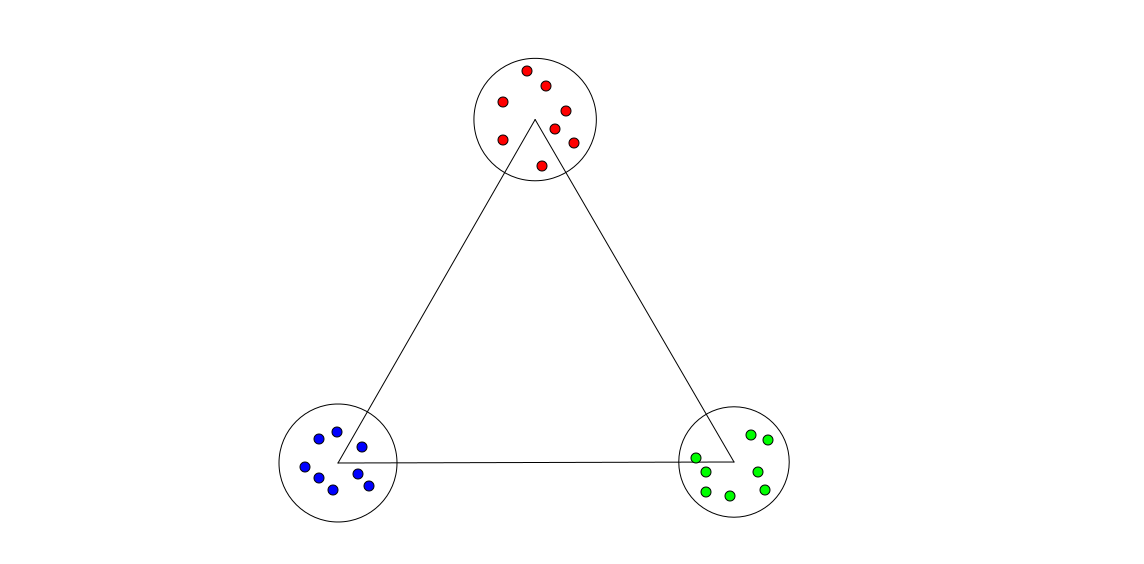
\includegraphics[keepaspectratio=true,width=\dimwidth{1.00},height=\dimheight{1.00}]{images/non_trivial_cut01}{}%mdk
%mdk
\end{mdframe}%mdk

%mdk-data-line={41}
\begin{mdframe}%mdk

%mdk-data-line={42}
\noindent\mdline{42}\includegraphics[keepaspectratio=true,width=\dimwidth{1.00},height=\dimheight{1.00}]{images/non_trivial_cut02}{}%mdk
%mdk
\end{mdframe}%mdk

%mdk-data-line={44}
\begin{mdframe}%mdk

%mdk-data-line={45}
\noindent\mdline{45}\includegraphics[keepaspectratio=true,width=\dimwidth{1.00},height=\dimheight{1.00}]{images/non_trivial_cut03}{}%mdk
%mdk
\end{mdframe}%mdk

%mdk-data-line={47}
\begin{mdframe}%mdk

%mdk-data-line={48}
\noindent\mdline{48}\includegraphics[keepaspectratio=true,width=\dimwidth{1.00},height=\dimheight{1.00}]{images/non_trivial_cut04}{}%mdk
%mdk
\end{mdframe}%mdk

%mdk-data-line={52}
\begin{mdframe}%mdk

\frametitle{Celdas el arreglos coloreados}\label{heading-sec-celdas-el-arreglos-coloreados}%mdk%mdk
%mdk
\end{mdframe}\label{sec-celdas-el-arreglos-coloreados}%mdk%mdk

%mdk-data-line={54}
\begin{mdframe}%mdk

\frametitle{En el plano}\label{heading-sec-en-el-plano}%mdk%mdk

%mdk-data-line={55}
\begin{mdbmarginx}{1ex}{0pt}{1ex}{0pt}%mdk
%mdk-data-line={56}
\noindent\mdline{56}\textbf{Theorem~1.} \mdbr
\mdline{56}  Sea \mdline{56}$L$\mdline{56} un conjunto 3 coloreado en el plano que induce un arreglo simple \mdline{56}$A(L)$\mdline{56}, talque
que cada color aparece al menos una ves. Entonces existe una \mdline{57}\emph{cara completa}\mdline{57} en \mdline{57}$A(L)$%mdk%mdk
\end{mdbmarginx}%mdk

%mdk-data-line={60}
\begin{mdbmarginx}{1ex}{0pt}{1ex}{0pt}%mdk
%mdk-data-line={61}
\noindent\mdline{61}\textbf{Lemma~1.} \mdbr
\mdline{61} Considera un ciclo simple donde cada vertice es coloreado con rojo, verde o azul. Entonces
 \mdline{62}$n_{rg} \equiv n_{rb} \equiv n_{gb} \mod 2$%mdk%mdk
\end{mdbmarginx}%mdk
%mdk
\end{mdframe}\label{sec-en-el-plano}%mdk%mdk

%mdk-data-line={65}
\begin{mdframe}%mdk

\frametitle{En dimensiones más grandes}\label{heading-sec-en-dimensiones-ms-grandes}%mdk%mdk

%mdk-data-line={66}
\begin{mdbmarginx}{1ex}{0pt}{1ex}{0pt}%mdk
%mdk-data-line={67}
\noindent\mdline{67}\textbf{Theorem~2.} \mdbr
\mdline{67}Sea \mdline{67}$L$\mdline{67} un conjunto de \mdline{67}$(d+1)$\mdline{67}-coloreados hyperplanos en \mdline{67}$I\!R^{d}$\mdline{67} que induce un arreglo simple
en \mdline{68}$A(L)$\mdline{68}, donde cada color aparece al menos una vez. Entonces existe una \mdline{68}\emph{cara completa}\mdline{68} en \mdline{68}$A(L)$%mdk%mdk
\end{mdbmarginx}%mdk

%mdk-data-line={71}
\begin{mdbmarginx}{1ex}{0pt}{1ex}{0pt}%mdk
%mdk-data-line={72}
\noindent\mdline{72}\textbf{Lemma~2.} \mdbr
\mdline{72}Considera una triangulación \mdline{72}$T$\mdline{72} en \mdline{72}$\mathbb{S}^{d-1}$\mdline{72} donde cada vertice es coloreado con un color
\mdline{73}{}[\mdline{73}$d$\mdline{73}]\mdline{73}. Entonces \mdline{73}$n_{s} \equiv 0(mod\ 2)$\mdline{73} para todos los \mdline{73}\emph{buenos tipos}\mdline{73} \mdline{73}$S$\mdline{73}, o
\mdline{74}$n_{s} \equiv 1 (mod\ 2)$\mdline{74} para todos los \mdline{74}\emph{buenos tipos}\mdline{74} \mdline{74}$S$\mdline{74}%mdk%mdk
\end{mdbmarginx}%mdk
%mdk
\end{mdframe}\label{sec-en-dimensiones-ms-grandes}%mdk%mdk

%mdk-data-line={77}
\begin{mdframe}%mdk

\frametitle{Conjunto de puntos 3 coloreados y cuñas balanceadas}\label{heading-sec-conjunto-de-puntos-3-coloreados-y-cuas-balanceadas}%mdk%mdk
%mdk
\end{mdframe}\label{sec-conjunto-de-puntos-3-coloreados-y-cuas-balanceadas}%mdk%mdk

%mdk-data-line={79}
\begin{mdframe}%mdk

%mdk-data-line={80}
\begin{mdbmarginx}{1ex}{0pt}{1ex}{0pt}%mdk
%mdk-data-line={81}
\noindent\mdline{81}\textbf{Theorem~3.} \mdbr
\mdline{81}Sea \mdline{81}$S$\mdline{81} un conjunto de puntos 3 coloreado en \mdline{81}$\mathbb{R}^{2}$\mdline{81} en posición general, donde cada
color aparece al menos una vez. Entonces existe un \mdline{82}\textbf{cuña}\mdline{82} que contiene exactamente un punto
de cada color de \mdline{83}$S$%mdk%mdk
\end{mdbmarginx}%mdk
%mdk
\end{mdframe}%mdk

%mdk-data-line={87}
\begin{mdframe}%mdk

%mdk-data-line={88}
\begin{mdbmarginx}{1ex}{0pt}{1ex}{0pt}%mdk
%mdk-data-line={89}
\noindent\mdline{89}\textbf{Theorem~4.} \mdbr
\mdline{89}Sea un conjunto 3 coloreado \mdline{89}\emph{balanceado}\mdline{89} de 6\mdline{89}$n$\mdline{89} puntos en \mdline{89}$\mathbb{R}^{2}$\mdline{89} en posición
general. Entonces existe una \mdline{90}\textbf{cuña}\mdline{90} que contiene exactamente n puntos de cada color de \mdline{90}$S$%mdk%mdk
\end{mdbmarginx}%mdk

%mdk-data-line={93}
\begin{mdbmarginx}{1ex}{0pt}{1ex}{0pt}%mdk
%mdk-data-line={94}
\noindent\mdline{94}\textbf{Corollary~1.} \mdbr
\mdline{94}Sea \mdline{94}$L$\mdline{94} un conjunto 3 coloreado balanceado de 6\mdline{94}$n$\mdline{94} lineas en \mdline{94}$\mathbb{R}^2$\mdline{94} que induce un 
arreglo simple. Entonces, siemple existe un segmento que intersecta exactamente \mdline{95}$n$\mdline{95} lineas
de cada color%mdk%mdk
\end{mdbmarginx}%mdk
%mdk
\end{mdframe}%mdk

%mdk-data-line={101}
\begin{mdframe}%mdk

\frametitle{Particiones balanceadas en curvas cerradas de Jordan}\label{heading-sec-particiones-balanceadas-en-curvas-cerradas-de-jordan}%mdk%mdk
%mdk
\end{mdframe}\label{sec-particiones-balanceadas-en-curvas-cerradas-de-jordan}%mdk%mdk

%mdk-data-line={103}
\begin{mdframe}%mdk

%mdk-data-line={104}
\begin{mdbmarginx}{1ex}{0pt}{1ex}{0pt}%mdk
%mdk-data-line={105}
\noindent\mdline{105}\textbf{Lemma~3.} \mdbr
\mdline{105}Para un entero fijo \mdline{105}$n \geq 2$\mdline{105} cualquier \mdline{105}$k \in \{1,2,...,n\}$\mdline{105} puede ser obtenido desde n
aplicando funciones \mdline{106}$f(x) = \lfloor x \rfloor$\mdline{106} y \mdline{106}$g(x)= n - x$\mdline{106} en a lo más \mdline{106}$2 \log n + O(1)$\mdline{106} tiempo%mdk%mdk
\end{mdbmarginx}%mdk
%mdk
\end{mdframe}%mdk

%mdk-data-line={110}
\begin{mdframe}%mdk

%mdk-data-line={111}
\begin{mdbmarginx}{1ex}{0pt}{1ex}{0pt}%mdk
%mdk-data-line={112}
\noindent\mdline{112}\textbf{Theorem~5.} \mdbr
\mdline{112}Sea \mdline{112}$\gamma$\mdline{112} un curva cerrada de Jordan en el plano, y sea \mdline{112}$P$\mdline{112} un conjunto 3 coloreado balanceado de \mdline{112}$3n$\mdline{112} puntos
en \mdline{113}$\gamma$\mdline{113}. Entonces para cada entero positivo \mdline{113}$k \leq n$\mdline{113} existe un \mdline{113}$2$\mdline{113}-arco conjunto \mdline{113}$P_{k} \subseteq \gamma$\mdline{113} 
que contiene exactamente \mdline{114}$k$\mdline{114} puntos de cada color.%mdk%mdk
\end{mdbmarginx}%mdk
%mdk
\end{mdframe}%mdk

%mdk-data-line={118}
\begin{mdframe}%mdk

\frametitle{$L$-lineas en el \emph{lattice}}\label{heading-sec-l-lineas-en-el--lattice-}%mdk%mdk
%mdk
\end{mdframe}\label{sec-l-lineas-en-el--lattice-}%mdk%mdk

%mdk-data-line={120}
\begin{mdframe}%mdk

%mdk-data-line={121}
\begin{mdbmarginx}{1ex}{0pt}{1ex}{0pt}%mdk
%mdk-data-line={122}
\noindent\mdline{122}\textbf{Definition~3.} ({\itshape L-linea})\mdbr%mdk%mdk
\end{mdbmarginx}%mdk

%mdk-data-line={123}
\begin{mdbmarginx}{1ex}{0pt}{1ex}{0pt}%mdk
%mdk-data-line={124}
\noindent\mdline{124}\textbf{Definition~4.} ({\itshape Posicion general en el Lattice})\mdbr%mdk%mdk
\end{mdbmarginx}%mdk
%mdk
\end{mdframe}%mdk

%mdk-data-line={128}
\begin{mdframe}%mdk

%mdk-data-line={129}
\begin{mdbmarginx}{1ex}{0pt}{1ex}{0pt}%mdk
%mdk-data-line={130}
\noindent\mdline{130}\textbf{Theorem~6.} \mdbr
\mdline{130}  Sea \mdline{130}$S$\mdline{130} un conjunto de puntos 3 coloreado balanceado de \mdline{130}$3n$\mdline{130} puntos en posicion general
  en el plano. Si el cierre convexo es \mdline{131}\emph{monocromatico}\mdline{131} entonces existe un linea de balanceo
  no trivial.%mdk%mdk
\end{mdbmarginx}%mdk
%mdk
\end{mdframe}%mdk

%mdk-data-line={136}
\begin{mdframe}%mdk

%mdk-data-line={137}
\begin{mdbmarginx}{1ex}{0pt}{1ex}{0pt}%mdk
%mdk-data-line={138}
\noindent\mdline{138}\textbf{Theorem~7.} \mdbr
\mdline{138}Sea \mdline{138}$S$\mdline{138} un conjunto 3 coloreado balanceado de \mdline{138}$3n$\mdline{138} puntos en posicion general en el \mdline{138}\emph{lattice}\mdline{138}.
Si el cierre ortogonal convezo de \mdline{139}$S$\mdline{139} es \mdline{139}\emph{monocromatico}\mdline{139}, entonces exita una \mdline{139}$L$\mdline{139}-linea de balanceo
no trivial.%mdk%mdk
\end{mdbmarginx}%mdk
%mdk
\end{mdframe}%mdk

%mdk-data-line={144}
\begin{mdframe}%mdk

\frametitle{Bibliografia}\label{heading-sec-bibliografia}%mdk%mdk

%mdk-data-line={145;out/3colBal-bib.bbl.mdk:1}
%mdk-data-line={145;out/3colBal-bib.bbl.mdk:2}
\mdsetrefname{References}%mdk
{\mdbibindent{0}%mdk
\begin{thebibliography}{1}%mdk
\label{sec-bibliography}%mdk

%mdk-data-line={science.bib:1}
\bibitem{bereg201521}\mdbibitemlabel{{}[1]}Sergey Bereg, Ferran Hurtado, Mikio Kano, Matias Korman, Dolores Lara, Carlos Seara, Rodrigo I.~Silveira, Jorge Urrutia, and Kevin Verbeek. \textquotedblleft{}Balanced Partitions of 3-Colored Geometric Sets in the Plane .\textquotedblright{} \emph{Discrete Applied Mathematics } 181: 21–32. 2015. doi:\href{https://dx.doi.org/10.1016/j.dam.2014.10.015}{10.1016/j.dam.2014.10.015}.\label{bereg201521}%mdk%mdk
\par%mdk
\end{thebibliography}}%mdk%mdk
%mdk
\end{mdframe}\label{sec-bibliografia}%mdk%mdk%mdk%mdk%mdk


\end{document}
